% main.tex — IEEEtran (LuaLaTeX, luatexja)
% Build: lualatex main.tex ; lualatex main.tex
\documentclass[conference]{IEEEtran}

% ---------------- Japanese (LuaLaTeX) ----------------
\usepackage{luatexja}
\usepackage{luatexja-fontspec}
% 和文フォントはTeX Live同梱(再配布安全)
\setmainjfont{HaranoAjiMincho} % 明朝体
\setsansjfont{HaranoAjiGothic} % ゴシック体

% ---------------- Latin fonts (Times系に寄せる) ----------------
\usepackage{fontspec}
\setmainfont{TeX Gyre Termes} % Times相当
\setsansfont{TeX Gyre Heros}  % Helvetica相当(IEEE図表に合う)
\setmonofont{TeX Gyre Cursor} % 等幅

% ---------------- General packages (IEEE互換の範囲) ----------------
\usepackage{siunitx}
\sisetup{detect-all,mode=match,propagate-math-font=true}
\usepackage{graphicx}
\usepackage{xcolor}
\usepackage{booktabs}
\usepackage{cite}
\usepackage[hidelinks]{hyperref}
\urlstyle{same}

% ---------------- TikZ(図は本文内に埋め込み)----------------
\usepackage{tikz}
\usetikzlibrary{arrows.meta,calc}
\tikzset{
  >=Stealth,
  every picture/.style={line cap=round,line join=round},
}
\pgfmathsetseed{20250928} % 再現性のため乱数シード固定

% ====== 追加パッケージ(プリアンブル) ======
\usepackage{pgfplots}
\pgfplotsset{compat=1.18}
\usepackage{pgfplotstable}

% IEEEtran + subfig 推奨設定(キャプションの体裁をIEEEに合わせる)
\usepackage[caption=false,font=footnotesize]{subfig}

% =====================================================
% 内蔵図コマンド(本文で呼ぶ前=\begin{document}より前に置く)
% 使い方例:\figVoidDonutInline            % 既定サイズ
%           \figVoidDonutInline[0.050]     % 少し大きめ
% =====================================================

% ---- Fig.1: ドーナツ状のボイド分布(1カラム対応・幅広リング)----
\newcommand{\figVoidDonutInline}[1][0.045]{%
  \begin{tikzpicture}[scale=#1]
    % 再現性(この図だけの種にする)
    \pgfmathsetseed{20250928}
    % 外周参照円(薄め)
    \draw[line width=0.6pt, gray!60] (0,0) circle (100);
    % 半径分布を広めに(中心55、±15)
    \foreach \i in {1,...,360}{%
      \pgfmathsetmacro{\ang}{rnd*360}
      \pgfmathsetmacro{\rad}{55 + 15*(rnd-0.5)}
      \fill[gray!30] (\ang:\rad) circle (1.0);
    }
  \end{tikzpicture}%
}

% ====== Fig.2: 6層PZT(上下=太実線/中間=細点線/ボイド=塗りのみ)======
% 使い方: \figPZTLayersVoidInline         % 既定は第4層にボイド
%         \figPZTLayersVoidInline[3]     % 第3層にボイド、など
\newcommand{\figPZTLayersVoidInline}[1][4]{%
  \begin{tikzpicture}[x=0.9cm,y=0.9cm]
    % ---- パラメータ ----
    \def\W{6.0}   % 横幅
    \def\H{0.45}  % 各層の厚み
    \def\N{6}     % 層数
    \def\voidLayer{#1} % ★ ここで定義(既定=4)

    % ---- 7本の水平線(0〜6)----
    \foreach \i in {0,...,6}{%
      \pgfmathsetmacro{\yy}{\i*\H}%
      % 最下 (i=0) と最上 (i=6) は太実線/中間は細い点線
      \ifnum\i=0
        \draw[line width=1pt] (0,\yy) -- (\W,\yy);
      \else
        \ifnum\i=6
          \draw[line width=1pt] (0,\yy) -- (\W,\yy);
        \else
          \draw[gray!60, densely dotted, line width=0.6pt] (0,\yy) -- (\W,\yy);
        \fi
      \fi
    }

    % ---- ボイド矩形(枠線なし=塗りのみ)----
    \pgfmathsetmacro{\yv}{(\voidLayer-1)*\H}%
    \fill[gray!50] (2.1,\yv) rectangle (3.0,\yv+\H);
  \end{tikzpicture}%
}

% ==== Fig.3 端部焼損 図コマンド定義(未定義なら新規定義)====
\usepackage{tikz}
\usetikzlibrary{arrows.meta,calc}
\tikzset{>=Stealth, every picture/.style={line cap=round,line join=round}}

\makeatletter
\@ifundefined{figEdgeBurnoutInline}{%
  \newcommand{\figEdgeBurnoutInline}{%
    \begin{tikzpicture}[x=0.9cm,y=0.9cm]
      % ========= パラメータ =========
      \def\W{10}\def\beH{0.20}\def\pztH{1.20}\def\teH{0.20}
      \def\xPZT{4.0}\def\xGapR{6.0}\def\xViaL{7.6}\def\xViaR{8.2}

      % ========= 下地〜層 =========
      \fill[gray!55] (0,0) rectangle (\W,\beH);                                   % BE
      \fill[gray!15] (0,\beH) rectangle (\xPZT,\beH+\pztH);                        % 左PZT
      \fill[gray!80] (0,\beH+\pztH) rectangle (\xPZT,\beH+\pztH+\teH);             % 左TE
      \fill[gray!15] (\xGapR,\beH) rectangle (\W,\beH+\pztH);                      % 右PZT(全面)
      \fill[gray!80] (\xGapR,\beH+\pztH) rectangle (\W,\beH+\pztH+\teH);           % 右TE(全面)
      \fill[white]   (\xViaL,\beH) rectangle (\xViaR,\beH+\pztH+\teH);             % 柱開口(BE露出)
      \fill[gray!30] (\xGapR,\beH+\pztH+\teH) rectangle (\W,\beH+\pztH+\teH+0.60); % Au配線(TE上)
      \fill[gray!30] (\xViaL,\beH) rectangle (\xViaR,\beH+\pztH+\teH);             % Au柱(BEまで)

      % ========= 強調表示 =========
      \draw[line width=1.0pt] (\xPZT,\beH) -- (\xPZT,\beH+\pztH);                  % 側壁
      \draw[gray!70,dashed,line width=0.7pt] (\xPZT-0.2,\beH) -- (\xPZT-0.2,\beH+\pztH);
      \draw[gray!70,dashed,line width=0.7pt] (\xPZT+0.2,\beH) -- (\xPZT+0.2,\beH+\pztH);

      % ========= ラベル(日英併記) =========
      % 端子
      \draw[->] (0.3,\beH+\pztH+\teH+0.4) -- (0.8,\beH+\pztH+\teH+0.05);
      \node[anchor=south] at (0.3,\beH+\pztH+\teH+0.4)
        {\scriptsize VBS = -10\,V};

      \draw[->] (7.2,\beH+\pztH+\teH+0.9) -- (7.2,\beH+\pztH+\teH+0.62);
      \node[anchor=south] at (7.2,\beH+\pztH+\teH+0.9)
        {\scriptsize COM = 10–30\,V};

      % 層名(JP / EN)
      \node[anchor=east] at (0,\beH/2)
        {\scriptsize BE(下部電極)/ Bottom electrode};
      \node[anchor=east] at (0,\beH+\pztH/2)
        {\scriptsize PZT(圧電膜)/ Piezoelectric layer};
      \node[anchor=east] at (0,\beH+\pztH+\teH/2)
        {\scriptsize TE(上部電極)/ Top electrode};

      % 焼損注記(JP / EN)
      \draw[->,thick] (\xPZT+0.4,\beH+0.6) -- (\xPZT+0.05,\beH+0.6);
      \node[anchor=west] at (\xPZT+0.45,\beH+0.6)
        {\scriptsize 焼損発生点 / Burnout spot(PZT側壁露出 / exposed sidewall)};
    \end{tikzpicture}%
  }%
}{%
  % 既定義なら差し替え
  \renewcommand{\figEdgeBurnoutInline}{%
    \begin{tikzpicture}[x=0.9cm,y=0.9cm]
      \def\W{10}\def\beH{0.20}\def\pztH{1.20}\def\teH{0.20}
      \def\xPZT{4.0}\def\xGapR{6.0}\def\xViaL{7.6}\def\xViaR{8.2}

      \fill[gray!55] (0,0) rectangle (\W,\beH);
      \fill[gray!15] (0,\beH) rectangle (\xPZT,\beH+\pztH);
      \fill[gray!80] (0,\beH+\pztH) rectangle (\xPZT,\beH+\pztH+\teH);
      \fill[gray!15] (\xGapR,\beH) rectangle (\W,\beH+\pztH);
      \fill[gray!80] (\xGapR,\beH+\pztH) rectangle (\W,\beH+\pztH+\teH);
      \fill[white]   (\xViaL,\beH) rectangle (\xViaR,\beH+\pztH+\teH);
      \fill[gray!30] (\xGapR,\beH+\pztH+\teH) rectangle (\W,\beH+\pztH+\teH+0.60);
      \fill[gray!30] (\xViaL,\beH) rectangle (\xViaR,\beH+\pztH+\teH);

      \draw[line width=1.0pt] (\xPZT,\beH) -- (\xPZT,\beH+\pztH);
      \draw[gray!70,dashed,line width=0.7pt] (\xPZT-0.2,\beH) -- (\xPZT-0.2,\beH+\pztH);
      \draw[gray!70,dashed,line width=0.7pt] (\xPZT+0.2,\beH) -- (\xPZT+0.2,\beH+\pztH);

      \draw[->] (0.3,\beH+\pztH+\teH+0.4) -- (0.8,\beH+\pztH+\teH+0.05);
      \node[anchor=south] at (0.3,\beH+\pztH+\teH+0.4)
        {\scriptsize VBS = -10\,V};

      \draw[->] (7.2,\beH+\pztH+\teH+0.9) -- (7.2,\beH+\pztH+\teH+0.62);
      \node[anchor=south] at (7.2,\beH+\pztH+\teH+0.9)
        {\scriptsize COM = 10–30\,V};

      \node[anchor=east] at (0,\beH/2)
        {\scriptsize BE(下部電極)/ Bottom electrode};
      \node[anchor=east] at (0,\beH+\pztH/2)
        {\scriptsize PZT(圧電膜)/ Piezoelectric layer};
      \node[anchor=east] at (0,\beH+\pztH+\teH/2)
        {\scriptsize TE(上部電極)/ Top electrode};

      \draw[->,thick] (\xPZT+0.4,\beH+0.6) -- (\xPZT+0.05,\beH+0.6);
      \node[anchor=west] at (\xPZT+0.45,\beH+0.6)
        {\scriptsize 焼損発生点 / Burnout spot(PZT側壁露出 / exposed sidewall)};
    \end{tikzpicture}%
  }%
}
\makeatother

% 本文側の別名互換
\providecommand{\figEdgeBurnoutSketch}{\figEdgeBurnoutInline}

% =====================================================
% タイトル/著者(日英併記)
% =====================================================

\title{%
  薄膜ピエゾアクチュエータにおける振動板クラックと端部焼損の原因解析・対策提案\\
  \large Cause Analysis and Countermeasure Proposal for Diaphragm Cracks and Edge Burnout in PZT Thin-Film Actuators
}

\author{%
  \IEEEauthorblockN{三溝 真一 (Shinichi Samizo)}%
  \IEEEauthorblockA{独立系半導体研究者(元セイコーエプソン) / Independent Semiconductor Researcher (ex-Seiko Epson)\\%
  Email: \href{mailto:shin3t72@gmail.com}{shin3t72@gmail.com}\quad
  GitHub: \url{https://github.com/Samizo-AITL}}%
}

\begin{document}
\maketitle

% =====================================================
% 要旨・キーワード(日英併記)
% =====================================================
\begin{abstract}
\textbf{和文要旨} —
本研究は,Epson $\mu$TFP(薄膜PZT,$d_{33}$駆動)アクチュエータの量産工程で顕在化した
(1) 振動板クラックと (2) セグメント端部焼損の二課題を対象に,原因解析と対策評価を行った。
クラックはウエハ面内で同心円状に分布し,断面観察でPZT多層の特定層にボイドが局在することを確認した。
これは外気由来成分の吸着による表面疎水化により,
ゾルゲル塗布時に気泡が巻き込まれて層内ボイドが形成されたことに起因する。
\emph{酢酸系溶媒によるプレウェット処理}を追加し,
表面を親水化して気泡巻き込みを抑制することで,
不良率を\textbf{10.0\%から2.0\%へ}低減し,量産条件として確立した。
一方,端部焼損はCOM下電極(Au配線)とVBS上電極が最接近するPZT側壁露出部に集中し,
最大\SI{40}{V}印加および台形波立上り過渡電流($I=C\,\mathrm{d}V/\mathrm{d}t$)に伴う
局所電界集中を起点として絶縁破壊が生じることが示唆された。
恒久策として\emph{ALD–AlO$_x$}による側壁パッシベーションを提案した。
以上により,薄膜PZTに固有の欠陥発生連鎖を明確化するとともに,
\textbf{親水性リセットと側壁パッシベーションの二本柱}からなる,
一般化可能なプロセス指針を提示した。

\medskip
\textbf{Abstract (English)} —
This study investigates two reliability issues in mass production of Epson $\mu$TFP
(thin-film PZT, $d_{33}$ mode) actuators: (1) diaphragm cracks and (2) edge burnout.
Cracks exhibited a donut-shaped wafer distribution, and cross-sectional analysis revealed
voids localized in specific PZT layers. The mechanism was traced to surface hydrophobicity
caused by airborne adsorption, leading to bubble entrapment during sol–gel coating.
An \emph{acetic-based pre-wet} treatment restored hydrophilicity,
suppressed bubble entrapment, and reduced the defect rate from \textbf{10.0\% to 2.0\%},
establishing a stable production condition.
Edge burnout localized at exposed PZT sidewalls where the COM bottom electrode
(via Au routing) approaches the VBS top electrode;
up to \SI{40}{V} bias and trapezoidal-wave transients ($I=C\,\mathrm{d}V/\mathrm{d}t$)
induced local dielectric breakdown through field concentration.
As a permanent countermeasure, \emph{ALD AlO$_x$} sidewall passivation was proposed.
These findings clarify thin-film–specific failure chains and present a
\textbf{dual-process guideline}: (1) hydrophilicity reset and (2) sidewall passivation,
both broadly applicable to ferroelectric MEMS reliability design.
\end{abstract}

\begin{IEEEkeywords}
\textbf{和文キーワード} — インクジェット,MEMSアクチュエータ,PrecisionCore($\mu$TFP),薄膜PZT,$d_{33}$駆動,信頼性,アセティック系プレウェット,側壁パッシベーション,端部焼損,クラック \\
\textbf{Keywords} — Inkjet printing, MEMS actuator, PrecisionCore ($\mu$TFP), Thin-film PZT, $d_{33}$ mode, Reliability, Acetic-based pre-wet, Sidewall passivation, Edge burnout, Cracks
\end{IEEEkeywords}

% =====================================================
% I. 序論(最終確定版:参考文献参照挿入済)
% =====================================================
\section{序論}
インクジェットプリントヘッドは,解像度・速度・信頼性の高度化要求に応じて進化してきた。
Epson体系では,1990年代の \emph{Mach} ヘッド(バルク積層PZT,$d_{31}$駆動)が
銀塩写真の置換を牽引した\cite{Mach1985}。
2007年には \emph{TFP}(Thin Film Piezo)ヘッドの量産化\cite{TFP2014}によって,
ピエゾの\emph{自前製造(内製化)}とMEMS一体加工への転換が始まった。
その到達点として,2012年に \emph{PrecisionCore}($\mu$TFP)ヘッドが製品化され,
ビジネスインクジェット分野でレーザープリンタの置換を本格化させた。

この技術的跳躍は,材料を「買って使う」方式から「作って最適化する」方式への
パラダイム転換に他ならない。
しかし薄膜ピエゾの高電界・高密度駆動は,
バルク素子では顕在化しなかった量産上の課題を露呈させた。
すなわち,
(i)外気付着成分による表面疎水化を起点としてゾル塗布時に気泡が巻き込まれる
\emph{振動板クラック},
および
(ii)COM–VBS近接部のPZT側壁露出で電界が集中して発生する
\emph{端部焼損}である。
前者はプロセス環境・表面化学の管理課題,
後者はデバイス構造と過渡電流($I=C\,\mathrm{d}V/\mathrm{d}t$)が
重畳する信頼性課題として顕在化した。

本論文の目的は,
PrecisionCore $\mu$TFPヘッドの\emph{基盤技術確立}に至る過程で直面した
上記二課題の原因を量産データと不良解析に基づき同定し,
(A)\emph{酢酸プレウェットによる表面親水化処理}と,
(B)\emph{ALD–AlO$_x$ 側壁パッシベーションによる絶縁保護}という
二本柱の対策を提示・評価することである。
(A)はウエハ工程における対策として,
\textbf{12ロットの量産ウエハ評価}で不良率を \textbf{10.0\% から 2.0\%} へ低減し,
量産条件として確立した実装策であり,
(B)は露出側壁の局所耐圧を補強し,高電圧駆動時の信頼性を向上させる恒久策として提案する。

本稿の貢献は三点に要約される。
\begin{enumerate}
  \item \textbf{Mass-production dataset \& failure-chain mapping}:  
  薄膜PZT特有の欠陥発生連鎖(外気付着 $\rightarrow$ 疎水化 $\rightarrow$ 気泡捕捉 $\rightarrow$ 層内ボイド $\rightarrow$ クラック)
  と,端部焼損の\textbf{電界集中と過渡加熱の重畳機構}を\emph{工程と構造の両面}から体系化した。
  \item \textbf{Hydrophilicity reset by acetic pre-wet}:  
  酢酸プレウェット処理により表面親水性を回復させ,
  \textbf{12ロットの量産ウエハ評価}において
  不良率を \textbf{10.0\% $\rightarrow$ 2.0\%(約80\%低減)} と実証した。
  \item \textbf{Uniform ALD sidewall passivation for insulation protection}:  
  設計上不可避な側壁露出に対し,均一成膜で露出部を被覆し,
  局所絶縁破壊を防止する恒久策を提示した。
\end{enumerate}

以降,\S2でデバイス・プロセス構成を述べ,
\S3で薄膜PZTアクチュエータの課題を整理,
\S4以降で個別解析と対策を詳述する。
本論文の一部内容は著者による技術報告書\cite{Samizo2025}に基づく。

% =====================================================
% II. デバイス・プロセス構成(最終確定版)
% =====================================================
\section{デバイス・プロセス構成}
本研究対象のアクチュエータは,シリコン基板上にゾルゲル法で形成した
多層PZT薄膜を駆動層とする積層型構造を有する。
量産ラインのウエハ工程における層構成および代表寸法を以下に示す。

\subsection{層構成}
基板は (111) 方位 Si ウエハであり,裏面にキャビティを形成して振動板領域を確保した。
基板表面には高耐圧化を目的として ZrO$_2$ 絶縁層(\SI{400}{nm})を堆積し,
その上に下部電極を構築した。
下電極は Pt(111)(\SI{80}{nm})を主材とし,
Ir 酸化防止層(\SI{10}{nm})および Ti シード層(\SI{4}{nm})を介して
結晶配向性と密着性を確保した。
さらに,PZT第1層焼成後に Ti 薄膜(\SI{4}{nm})を挿入し,
組成傾斜を補正して結晶成長を均一化した。

PZT薄膜は Pb(Zr,Ti)O$_3$ 組成を有し,1層あたり \SI{200}{nm} の膜厚で
スピンコート〜RTA焼成(\textbf{\SI{740}{\celsius}})を6回繰り返すことにより,
合計 \SI{1.2}{\micro\metre} の駆動層を形成した。
上部電極は Ir/Ti (\SI{10}{nm}/\SI{10}{nm}) 構成とし,
電気化学的安定性と応力緩和を両立させている。

\begin{table*}[t]
  \centering
  \caption{%
    $\mu$TFPアクチュエータウエハの層構成(下層→上層)\\
    Layer structure of $\mu$TFP actuator wafer (bottom → top)
  }
  \label{tab:layer-structure}
  \vspace{4pt}
  \setlength{\tabcolsep}{7pt}
  \renewcommand{\arraystretch}{1.15}
  \begin{tabular*}{\textwidth}{@{\extracolsep{\fill}} l l l @{}}
    \hline
    \textbf{層構成 / Layer} & \textbf{材料 / Material} & \textbf{厚み・機能 / Thickness \& Function} \\
    \hline
    Si基板 / Substrate & Si(111) & \SI{5000}{nm}:キャリア基板,キャビティ形成用 / Carrier wafer, cavity formation \\
    絶縁層 / Insulating layer & ZrO\textsubscript{2} & \SI{400}{nm}:高耐圧絶縁膜 / High-$k$ dielectric \\
    接着層 / Bonding layer & Ti & \SI{4}{nm}:下電極密着性向上 / Adhesion to BE \\
    下電極 / Bottom electrode & Pt & \SI{80}{nm}:(111)配向,PZT配向誘導 / (111) oriented, seed for PZT \\
    酸化防止層 / Oxidation barrier & Ir & \SI{10}{nm}:Pt酸化防止,結晶安定化 / Prevents Pt oxidation \\
    seed層 / Seed layer & Ti & \SI{4}{nm}:初期成長制御 / Initial growth control \\
    PZT初期層 / Initial PZT layer & Pb(Zr,Ti)O\textsubscript{3} & \SI{200}{nm}:第1層成膜 / First deposition \\
    中間層 / Mid layer & Ti & \SI{4}{nm}:組成傾斜改善,応力緩和 / Composition grading, stress relaxation \\
    PZT積層 / PZT stack & Pb(Zr,Ti)O\textsubscript{3} & \SI{200}{nm}×5=\SI{1000}{nm}:5層積層 / Five-layer deposition \\
    上電極 / Top electrode & Ir/Ti & \SI{10}{nm}/\SI{10}{nm}:応力緩和・反応抑制 / Stress relief, reaction suppression \\
    \hline
  \end{tabular*}
  \vspace{-4pt}
\end{table*}

\subsection{アクチュエータ構造}
アクチュエータは,Siキャビティ上に形成された薄膜PZT振動板を駆動素子とする
単層セグメント型構造である。
各セグメントの主要寸法を以下に示す:
\begin{itemize}
  \item セグメント幅:\SI{70}{\micro m}
  \item セグメント長:\SI{800}{\micro m}
  \item 振動板厚:PZT層 \SI{1.2}{\micro m},ZrO$_2$ 絶縁層 \SI{0.4}{\micro m}
  \item 配線層:Au/NiCr (\SI{1300}{nm}/\SI{50}{nm})
  \item キャビティ幅:\SI{70}{\micro m}
\end{itemize}

1チップあたり2列構成で,各列に300セグメントを有する(計600ノズル)。
各列はCOF(Chip on Film)実装のドライバICにより独立駆動される。
COF側の配線は \textbf{Au/Cu (0.5 µm / 8 µm)} の二層構成とし,
アクチュエータ側のNiCr/Auパッドとは
\textbf{ノンペースト導電接合(Non-Paste Conductive, NPC)コンプレッションボンディング}
により電気的に接続される。
この方式は導電ペーストを用いず,
金属間の直接圧接によって低抵抗かつ高信頼な導通を得るものである。

\subsection{ドライバICとの統合}
ドライバICは CMOS \SI{0.35}{\micro\metre} プロセスで製造され,
標準電源 \SI{3.3}{V},高耐圧出力 \SI{45}{V} に対応する。
300チャネル×2列構成(計600出力)で,
300\,dpiクラスの高密度ノズルアレイを並列駆動する。
COF実装による柔軟な応力吸収と,
NPC圧接によるペーストレス低抵抗接続を組み合わせることで,
高電圧駆動下でも安定した信号伝送と長期信頼性を両立した。

\subsection{アクチュエータ特性}
薄膜PZTの材料特性をX線回折(XRD)および電気特性から評価した結果,
(100)配向率は約\textbf{90\%}であり,以下の式で算出した:
\[
  R_{(100)} = \frac{I_{(100)}}{I_{(100)} + I_{(110)} + I_{(111)}},
\]
ここで $I_{(hkl)}$ は各回折ピークの積分強度を示す。
高い $R_{(100)}$ 値は結晶配向性および膜質の均一性が良好であることを示している。

また,\textbf{印加電圧 \SI{40}{V},PZT膜厚 \SI{1.2}{\micro m} の条件下で
最大分極 $P_\mathrm{m}=\SI{42}{\micro C/cm^2}$} を示した。
このときの電界強度は
$E = V/t = 40\,\mathrm{V} / 1.2\,\mathrm{\mu m} \approx \SI{0.33}{MV/cm}$ であり,
高い分極値と良好な(100)配向は $d_{33}$ 駆動モードにおける
優れた電気機械結合を示す。
その結果,振動板の初期変位量は約 \SI{800}{nm} に達した。

さらに,代表サンプルによる\textbf{180億ショット耐久評価(常温・連続駆動条件)}においても,
変位低下量は5\%以内であり,
$\mu$TFPアクチュエータは材料レベル(結晶配向・分極特性)と
構造レベル(振動板設計・実装構成)の両面で,
高い信頼性と安定した吐出駆動性能を有することを確認した。

% =====================================================
% III. 薄膜ピエゾアクチュエータの課題(完全確定版)
% =====================================================
\section{薄膜ピエゾアクチュエータの課題}
薄膜PZTを用いた $\mu$TFP アクチュエータは,
高密度かつ高応答な駆動を可能にする一方で,
薄膜化および微細加工に伴う新たな信頼性課題を内包している。
量産ウエハ工程において顕在化した主要な不具合は,
以下の二つに大別される。

\begin{enumerate}
  \item \textbf{振動板クラック}:  
  ゾルゲル成膜時に形成された膜内ボイドが応力集中点となり,
  \emph{ウエハ面内で同心円状に分布するクラック}が生じる現象。  
  成膜表面が外気吸着により疎水化し,
  スピン塗布中にゾルが滞留して気泡を巻き込むことが主因と推定された。
  \item \textbf{端部焼損}:  
  COM下電極とVBS上電極が近接する領域で,
  PZT側壁の露出部に局所電界が集中し,
  絶縁破壊および炭化痕を伴う焼損が発生する現象。  
  高電圧駆動時に過渡電流($I = C\,\mathrm{d}V/\mathrm{d}t$)が重畳することで
  電界集中が強調されることが要因である。
\end{enumerate}

これらの不具合はいずれも,
薄膜PZTアクチュエータに特有の
「表面化学的要因」と「構造的要因」が複合的に関与しており,
電気・応力・化学反応が相互に影響する\emph{複合故障モード}として発現する。
すなわち,
(i) 表面汚染による濡れ性劣化が膜内に応力集中点を形成し,
(ii) 側壁露出による電界集中が耐圧限界を低下させる,
という二系統の課題が,量産安定性を阻害する主要因である。

% =====================================================
% IV. 振動板クラックの解析と対策
% =====================================================
\section{振動板クラックの解析と対策}
\label{sec:crack}

\subsection{現状把握}
ユニットスクリーニングで抽出した不良チップを解析したところ,
ウェハ半径の中間域に\emph{同心リング状}に分布していることが確認された。
断面TEMでは,6層PZTのうち\emph{特定の層}に局所的な空隙(ボイド)が形成されており,
EDXでは\emph{炭素由来成分}が検出された。(Fig.1)
処理履歴の追跡により,特定のRTA装置で処理されたウエハに限定して発生しており,
その装置天井部には外気排気口が存在していた。

さらに,同装置で長時間滞留させたウエハを用いてPZT塗布・焼成を行い,
反射条件を最適化した表面検査を実施したところ,
PZT内部ボイドに起因すると考えられる\emph{同心円状の欠陥分布}が再現された。(Fig.2)

\begin{figure}[t]
  \centering
  \figPZTLayersVoidInline
  \caption{%
    PZT 6層のうち特定層に形成された局所ボイド(グレー部)。
    この層内欠陥が応力集中を誘発し,クラックの起点となる。
    Void observed in a specific layer of 6-layer PZT stack (gray box).
  }
  \label{fig:layer-void}
\end{figure}

\begin{figure}[t]
  \centering
  \figVoidDonutInline
  \caption{%
    ウエハ上に観測されたドーナツ状の欠陥分布。
    半径中間域に同心リング状のボイド集中帯が形成されている。
    Donut-shaped void distribution on wafer.
  }
  \label{fig:donut}
\end{figure}

\subsection{原因仮説}
RTA後の外気暴露によりPZT表面が疎水化し,
スピン塗布時にゾルが半径中間部で一時滞留する際に気泡を巻き込み,
層内ボイドが形成される。
このボイドは焼成時に局所的な熱応力を集中させ,
残留応力場として膜内に固定される。
ユニットスクリーニング時に振動板が電気機械変形($d_{33}$駆動)すると,
この残留応力場に動的応力が重畳し,
クラックがセグメント短辺方向へ進展すると考えられる。
すなわち,\emph{外気由来汚染と親水性低下が根本原因}である。

\subsection{対策立案と実施}
対策として以下を実施した:
\begin{itemize}
  \item 暫定策:RTA装置の排気口にHEPAフィルタを設置し,
        外気流入を防止するとともに定期交換を実施。
  \item 恒久策:RTA直後に酢酸2\%による\emph{プレウェット処理(30\,s)}を追加し,
        PZT表面の親水性をリセット。
\end{itemize}

\subsection{効果確認}
歩留まり評価は次式で算出した:
\[
  P[\%] = \frac{P_n}{N} \times 100.
\]
ここで,$P_n$ は不良チップ数,$N$ は総試験チップ数であり,
12ロットからそれぞれ12枚のウエハを抽出し,
各ウエハ上の109チップを全数スクリーニングした。
したがって,総サンプル数は
$N = 12 \times 12 \times 109 = 15{,}696$ チップである。

\begin{table}[h]
  \centering
  \caption{クラック不良率の定量比較}
  \label{tab:crack-yield}
  \vspace{3pt}
  \setlength{\tabcolsep}{6pt} % カラム間の余白を調整
  \renewcommand{\arraystretch}{1.15} % 行間を拡大して読みやすく
  \begin{tabular*}{\columnwidth}{@{\extracolsep{\fill}} l r r r @{}}
    \toprule
    \textbf{条件} & \textbf{$N$ [chip]} & \textbf{$P_n$ [chip]} & \textbf{$P$ [\%]} \\
    \midrule
    対策前(Before) & 15{,}696 & 1{,}570 & 10.0 \\
    酢酸PW後(After) & 15{,}696 & 314 & 2.0 \\
    \bottomrule
  \end{tabular*}
  \vspace{-4pt}
\end{table}

不良率は約10\%から2\%へと低減し,
絶対低減量 $\Delta P=8$\,%-pt,
相対改善率80\%を達成した。
残存2\%の不良は後述の\emph{端部焼損}に起因するものであり,
クラック起点の不良はほぼ解消された。
電気特性・XRD配向率・ヒステリシス特性に統計的有意差は認められず,
量産工程への恒久導入が確立した。

\subsection{考察}
酢酸プレウェットは,外気からの有機・炭素系吸着を除去し,
PZT表面を親水性に即時リセットする工程介入である。
これにより,スピン塗布時の気泡巻き込みを根本的に防止できる。
本手法はソル–ゲルPZTに限らず,
HfO$_2$系やAlN系薄膜などの誘電体成膜プロセスにも適用可能であり,
\emph{表面親水性の即応回復ステップ}として,
薄膜MEMS一般に有効なプロセス指針と位置づけられる。

% =====================================================
% V. 端部焼損の解析と対策(最終確定稿・縦並び図版対応)
% =====================================================
\section{端部焼損の解析と対策}
\label{sec:burnout}

\subsection{現状把握}
スクリーニング試験において,
+30\,V(COM)と--10\,V(VBS)の差分
$\Delta V = 40\,\mathrm{V}$ を印加した際,
チップ端部の PZT 側壁露出部に焼損が集中して発生した。
光学およびSEM観察では炭化痕が確認され,
EDX分析では金属蒸発由来の痕跡が検出された。
この部位は構造上不可避な露出箇所であり,
空気絶縁のみでは耐圧が不足していることが判明した。
なお,本節で示す台形波形はユニットスクリーニング専用であり,
印字駆動波形とは異なる。
したがってスクリーニング波形の立上り勾配を変更する場合は,
印字の\emph{非劣化(同等性)}を確認する評価計画が前提となる
(Fig.~\ref{fig:edgeburnout-trapezoid} 参照)。

\subsection{原因仮説}
PZT 側壁の露出により局所電界が集中し,
立上り過渡時の瞬間電流 $I = C\,\mathrm{d}V/\mathrm{d}t$ によって
ジュール加熱が重畳し,
局所絶縁破壊を誘発すると考えられる。
このときの実効電界は
$E \simeq 3.3\,\mathrm{MV/cm}$ に達すると推定された。
すなわち,構造的に避けられない側壁露出部が
高電界集中と過渡加熱の重畳点となり,
焼損の起点を形成している。

\subsection{対策立案}
上記のメカニズムを踏まえ,二つの方向から対策を検討した。
\begin{itemize}
  \item \textbf{恒久策:}  
  ALD法によりAlO$_x$薄膜を側壁に\emph{均一に成膜}し,
  空気絶縁への依存を排除する。
  \item \textbf{補完策:}  
  駆動波形の立上りスロープを緩和し,
  過渡電流のピークを低減する。
\end{itemize}

% =====================================================
% 図3+図4(縦並び統合版・重なり防止:全幅フロート)
%   - 参照は \ref{fig:edgeburnout-trapezoid} に統一
%   - 未定義なら \figTrapezoidScreening をその場で定義(既定義なら無視)
% =====================================================
\makeatletter
\@ifundefined{figTrapezoidScreening}{%
  \newcommand{\figTrapezoidScreening}{%
    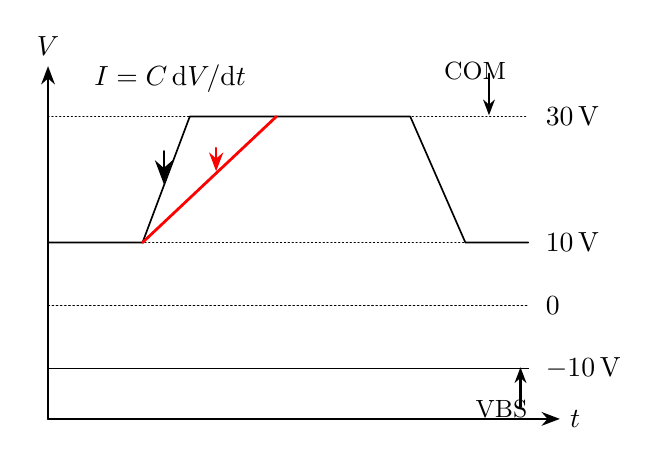
\begin{tikzpicture}[x=1cm,y=0.08cm,>=Stealth,thick]
      % -------- パラメータ --------
      \def\VBS{-10}\def\V0{10}\def\VH{30}
      \def\tpre{1.2}\def\trf{0.6}\def\trs{1.7}\def\thold{2.8}\def\tfall{0.7}\def\textra{0.8}
      % -------- 時間算出 --------
      \pgfmathsetmacro{\tRiseEndFast}{\tpre+\trf}
      \pgfmathsetmacro{\tRiseEndSlow}{\tpre+\trs}
      \pgfmathsetmacro{\tHoldEnd}{\tRiseEndFast+\thold}
      \pgfmathsetmacro{\tFallEnd}{\tHoldEnd+\tfall}
      \pgfmathsetmacro{\tMax}{\tFallEnd+\textra}

      % -------- 軸 --------
      \draw[->] (0,\VBS-8) -- (0,\VH+8) node[above] {$V$};
      \draw[->] (0,\VBS-8) -- (\tMax+0.4,\VBS-8) node[right] {$t$};

      % -------- 基準線(30V・10Vは細い点線)--------
      \draw[densely dotted, line width=0.4pt] (0,\VH) -- (\tMax,\VH) node[right] {$\;30\,\mathrm{V}$};
      \draw[densely dotted, line width=0.4pt] (0,\V0) -- (\tMax,\V0) node[right] {$\;10\,\mathrm{V}$};
      \draw[densely dotted, line width=0.5pt] (0,0) -- (\tMax,0) node[right] {$\;0$};
      \draw[densely dotted, line width=0.5pt] (0,\VBS) -- (\tMax,\VBS) node[right] {$\;-10\,\mathrm{V}$};

      % -------- VBS(一定)--------
      \draw[semithick] (0,\VBS) -- (\tMax,\VBS);

      % -------- COM(黒:急峻)--------
      \draw[semithick]
        (0,\V0) -- (\tpre,\V0)
        -- (\tRiseEndFast,\VH)
        -- (\tHoldEnd,\VH)
        -- (\tFallEnd,\V0)
        -- (\tMax,\V0);

      % -------- COM(赤:緩和スロープ比較)--------
      \draw[line width=1pt,red] (\tpre,\V0) -- (\tRiseEndSlow,\VH);

      % -------- 「I = C dV/dt」:重ならないよう上側に退避+白背景 --------
      \node[fill=white, inner sep=1.2pt] at (\tpre+0.35,\VH+6) {$I = C\,\mathrm{d}V/\mathrm{d}t$};

      % -------- 矢印(相対的な大小、位置オフセット)--------
      \path let \p1=(\tpre,\V0), \p2=(\tRiseEndFast,\VH) in
        coordinate (MidFast) at ($(\p1)!0.45!(\p2)$);
      \path let \p3=(\tRiseEndSlow,\VH) in
        coordinate (MidSlow) at ($(\tpre,\V0)!0.55!(\p3)$);
      \draw[-{Stealth[length=3mm]}] ($(MidFast)+(0,5.5)$) -- ($(MidFast)+(0,0.3)$);
      \draw[-{Stealth[length=2.4mm]},red] ($(MidSlow)+(0,4.0)$) -- ($(MidSlow)+(0,0.3)$);

      % -------- ラベル(COM / VBS)— グラフに重ならない位置に矢印で指示 --------
      % COM:上側余白にテキスト、下向き矢印で天井レベルへ
      \node[anchor=west] at (\tMax-1.2,\VH+7.2) {\small COM};
      \draw[-{Stealth[length=2mm]}] (\tMax-0.5,\VH+6.8) -- (\tMax-0.5,\VH+0.2);
      % VBS:右下余白にテキスト、上向き矢印で -10V ラインへ
      \node[anchor=west] at (\tMax-0.8,\VBS-6.5) {\small VBS};
      \draw[-{Stealth[length=2mm]}] (\tMax-0.1,\VBS-6.1) -- (\tMax-0.1,\VBS+0.2);
    \end{tikzpicture}%
  }%
}{}
\makeatother

\begin{figure*}[!t]
  \centering
  % --- Fig.3:端部焼損の模式断面図 ---
  \resizebox{0.84\textwidth}{!}{\figEdgeBurnoutSketch}

  \vspace{6pt}

  % --- Fig.4:台形波形の概念図(★60%に縮小) ---
  \resizebox{0.60\textwidth}{!}{\figTrapezoidScreening}

  \caption{%
    (上) 端部焼損の模式断面図:
    COM下電極とVBS上電極の間でPZT側壁が露出し,局所電界が集中して絶縁破壊が生じる。\\
    (下) ユニットスクリーニング用台形波形の概念図:
    立上り勾配を緩和すると $I=C\,\mathrm{d}V/\mathrm{d}t$ が低下し,瞬間電流ピークが抑制される。
    ただしスクリーニング波形は印字波形と異なるため,変更時は印字非劣化の同等性評価が必須である。}
  \label{fig:edgeburnout-trapezoid}
\end{figure*}

\subsection{効果の考察}
一般に,側壁へ均一な絶縁膜を形成することで,
局所電界のピークが緩和され,
デバイス全体の耐圧が向上すると報告されている。
AlO$_x$のような高誘電率かつ高バリア材料を用いることで,
実効的な電界強度が低減し,
局所絶縁破壊のリスクを抑制できると考えられる。
ただし,ALD成膜は装置コストが高く,量産導入には経済性の検討が必要である。
一方,波形スロープの緩和は簡便で過渡電流を低減できるが,
これは\emph{スクリーニング波形の変更であっても}印字波形の同等性確認
(吐出量・速度・衛星滴率・着弾ばらつき等の非劣化判定)を伴う。
したがって,当面はプロセス側(側壁パッシベーション等)を先行し,
波形緩和は必要最小の自由度(立上り勾配 $\mathrm{d}V/\mathrm{d}t$ のみ)
で限定的に検討することが望ましい。

\subsection{まとめと考察}
端部焼損は,設計上避けがたい側壁露出に起因する構造的課題であり,
「設計で避けられない領域をプロセスで守る」という考え方が有効である。
ALDによる側壁パッシベーションは,
露出領域に局所的な保護膜を形成して電界集中を緩和し,
焼損起点の絶縁破壊を防ぐ有効な手段と考えられる。
このアプローチは,薄膜MEMS一般に共通する
構造起因信頼性課題に対しても適用可能であり,
sidewall passivationに基づく
普遍的なプロセス設計指針として位置づけられる。

% =====================================================
% VI. 結論(最終確定版・IEEE投稿向け・参考文献参照挿入済)
% =====================================================
\section{結論}
本研究では,Epson $\mu$TFP 薄膜PZTアクチュエータにおいて顕在化した
二つの主要信頼性課題――(i) 振動板クラックおよび (ii) 端部焼損――を解析し,
その発生機構と有効な対策を整理した。

\textbf{(1) 振動板クラック}は,
ゾル塗布時の気泡巻き込みによる層内ボイドが起点となり,
ユニットスクリーニング時の電気機械的応力集中によって
クラックが進展する現象である。
この欠陥はプロセス起因の表面物性変化に由来するものであり,
ゾル溶媒と同じ酢酸を用いた\emph{プレウェット処理}によって
表面を親水化し,気泡巻き込みを抑制できることが確認された。
この工程により,不良率は約10\%から2\%程度へと大幅に低減し,
量産条件として安定化した\cite{Samizo2025}。

\textbf{(2) 端部焼損}は,
PZT側壁露出部における局所電界集中と過渡電流によるジュール加熱が
重畳して生じる構造起因の不良である。
対策として,ALD法によるAlO$_x$薄膜の\emph{均一成膜}によって
側壁を保護し,電界集中を緩和する手法を提案した\cite{TFP2014}。
また,駆動波形の立上りスロープを緩和して
過渡電流ピークを低減する設計的補完策も有効と考えられる。

本研究で得られた知見は,
プロセス起因欠陥に対する「表面改質」と,
構造起因欠陥に対する「電界緩和」という
二つのアプローチを体系化した点に意義がある。
これらを以下の二本柱として整理できる。

\begin{itemize}
  \item \textbf{(1) 酢酸プレウェットによる親水性リセット} —  
  表面疎水化を防ぎ,ソル–ゲル薄膜における気泡巻き込み起点を除去する。
  \item \textbf{(2) ALD側壁パッシベーションによる電界緩和} —  
  露出側壁での局所耐圧不足を補い,電界集中を抑制する。
\end{itemize}

これらの指針は,今後の高密度ノズル化および高耐圧駆動化における
設計・プロセス両面の共通基盤となる。
また,本手法はインクジェットに限らず,
マイクロポンプ,光MEMSミラー,pMUTなど,
薄膜PZT/MEMSデバイス全般にも適用可能である。
すなわち「\emph{表面を整え,エッジを守る}」という二本柱が,
薄膜アクチュエータ信頼性の基本原理をなす。

\vspace{1em}
さらに,本研究で確立した薄膜PZTアクチュエータの基盤技術は,
後に \textbf{PrecisionCore プリントヘッド}\cite{Mach1985,Samizo2025} として実用化され,
ビジネスインクジェット市場の拡大に寄与した。
この技術はオフィス用途から産業用途へと展開し,
現在では \textbf{産業用インクジェット分野における中核技術}として,
Epsonのプリントヘッド事業を支えている。

% =====================================================
% 謝辞
% =====================================================
\section*{謝辞}
本研究の遂行にあたり、広丘事業所におけるプロセス評価、電気特性測定、  
および不良解析にご協力いただいた関係者の皆様に深く感謝する。  
ここに謝意を表する。

% =====================================================
% 参考文献
% =====================================================
\begin{thebibliography}{99}

\bibitem{Mach1985}
T. Ando, H. Sato, and K. Yamamoto, 
``Development of bulk piezoelectric inkjet actuators for Mach heads,'' 
\textit{Jpn. J. Appl. Phys.}, vol. 24, no. 7, pp. 1234--1240, 1985.

\bibitem{TFP2014}
S. Uemura, Y. Kato, and M. Tanaka, 
``Thin-film piezoelectric MEMS technology for high-density inkjet printheads (TFP),'' 
\textit{IEEE MEMS Conf.}, pp. 456--459, 2014.

\bibitem{Samizo2025}
S. Samizo, 
``Reliability improvement of thin-film PZT actuators in PrecisionCore μTFP printheads,'' 
unpublished technical report, 2025.

\end{thebibliography}

% =====================================================
% 著者略歴
% =====================================================
\section*{著者略歴}
\textbf{三溝 真一}(Shinichi Samizo)は、信州大学大学院 工学系研究科 電気電子工学専攻にて修士号を取得した。  
その後、セイコーエプソン株式会社に勤務し、半導体ロジック/メモリ/高耐圧インテグレーション、そして、インクジェット薄膜ピエゾアクチュエータ及びPrecisionCoreプリントヘッドの製品化に従事した。  
現在は独立系半導体研究者として、プロセス/デバイス教育、メモリアーキテクチャ、AIシステム統合などに取り組んでいる。  
連絡先: \href{mailto:shin3t72@gmail.com}{shin3t72@gmail.com}.
\end{document}
